\documentclass{article}

\usepackage[T1]{fontenc}
\usepackage[utf8]{inputenc}
\usepackage[french,english]{babel}

%% This package is necessary to use \includegraphics.
\usepackage{graphicx}

%% This package is necessary to define hyperlinks.
\usepackage{hyperref}

%% These packages are necessary to include code.
\usepackage{listings}
\usepackage{minted} % colored

%% This package is needed to enchance mathematical formulas.
\usepackage{amsmath}



% This is a comment line in latex

% Latex allows you to define your own "commands",
% better known as "macros" in the Latex world.
% The following line is an example of such definition.
\newcommand{\latex}{\LaTeX}


% The next lines contain some meta informations about this document.

\title{Rapport Projet Long\\ Pour le 15 mars 2023}
%\subtitle{A minimal demonstration of \latex}

\author{Ange Herman KOUE-HEMAZRO, Eric NZABA}


%% Here we begin giving the actual content o the document.
\begin{document}
\maketitle

\selectlanguage{french}

\section{Introduction}
\paragraph{But du projet.} Implémenter une IA pour le jeu d'echecs basée sur la Recherche 
arborescente Monte-Carlo.

\paragraph{Métrique.} A l'aide de l'API Lichess.org, nous pouvons omettre l'implémentation d'une interface graphique pour notre jeu d'échec. L'API permet aussi de directement évalué les performances de notre algorithme face à l'IA Stockfish du site. Afin d'évaluer la réussite du projet, nous aimerions que notre algorithme puisse vaincre au moins les 3 premiers niveaux de l'IA Stockfish.
L'algorithme de Monte Carlo se base sur du hasard, il faudra trouver des stratégies afin de pouvoir d'augmenter les chances de victoire contre l'IA.
Nous pourrons ensuite déterminer un pourcentage de victoire à l'aide de plusieurs simulations.

\section{Implementation}
\paragraph{Comment on réalise notre projet.} 
Le projet est realisé en Python, on utilise l'API de Lichess.org afin d'éviter d'implémenter la partie du graphique du jeu comme convenu avec les professeurs.

\paragraph{Logiciel déjà codé} . La représentation du jeu d'échec est codé, les mouvements des pièces. En revanche il reste certaines spécificités du jeu d'échec à implémenter (Le coup en passant, les ex-aequo) Les fonctions vérifiant la sécurité du roi ne fonctionne pas de manière consistente.
La connexion avec l'API a été coder, ainsi que l'algorithme de Monte Carlo (à compléter...). Nous pouvons donc lancer l'IA contre un bot Stockfish.

\paragraph{Structure en modules/packages.} Nous avons 3 packages sans compter le package des tests. Le
package {\tt ai} est celui qui contient les fichiers en rapport avec notre IA basé sur Monte Carlo. Le package
{\tt api} quant à lui contient tout ce qui est en rapport avec l'API de lichess.org, les fonctions de connexions,
de récupération et d'envoie de données etc. Enfin le package {\tt chess} contient tout ce qui est en rapport avec
notre représentation du jeu d'echecs, les fonctions pour avoir tous les coups possibles etc ...

\paragraph{Représentation des données.} Initialement, nous avons representé le plateau de jeu comme un tableau d'entier afin d'optimiser la vitesse des opérations sur celui-ci mais aussi minimiser la taille de stockage dans la mémoire. En effet étant donné que notre algorithme effectue une multitude de simulation sur plusieurs plateau de jeu différent, nous avions considéré qu'il était judicieux de prioriser des coûts d'opérations et un stockage stockage minime.En revanche, suite à quelques difficultés rencontrés, nous avons déterminé que la representation en objet pouvait faciliter l'implémentation de plusieurs principe du jeu d'échec, comme par exemple le roque, ou la mise en danger du roi.   
Plus tard, nous introduirons un fichier stockant les meilleurs ouvertures afin que notre IA puisse en selectionner depuis celui-ci.

\paragraph{Technologies sur lesquelles notre code s'appuie.} Notre IA se base sur l'algorythme de recherche arborescente Monte Carlo et nous utilisons aussi l'api de lichess.org pour la partie graphique.

\section{Jalons}

\paragraph{Tâches à realiser pour conclure le projet.} 
\begin{enumerate}
  \item Régler les bugs dans les mouvements des pièces
  \item Changer la conception en rajoutant des objets pieces
  \item Faire un bon calcul de l'etat pour un bon choix des coups
  \item Permettre à un utilisateur lambda de jouer contre notre IA
  \item Simulation de  plusieurs parties contre les bots de Lichess pour sortir les pourcentages de victoires
\end{enumerate}
\paragraph{Tâches déja terminées.}
\begin{enumerate}

  \item Partie de l'api qui permet à notre IA de jouer contre celles de lichess
  \item Implémentation de l'algorithme de recherche arborescente Monte Carlo
  \item Implémentaion des mouvements d'échecs sauf celui du roi ( Encore quelques bugs)
\end{enumerate}

\paragraph{Organisation temporelle des tâches.}

\begin{figure}[ht]
  \centering
  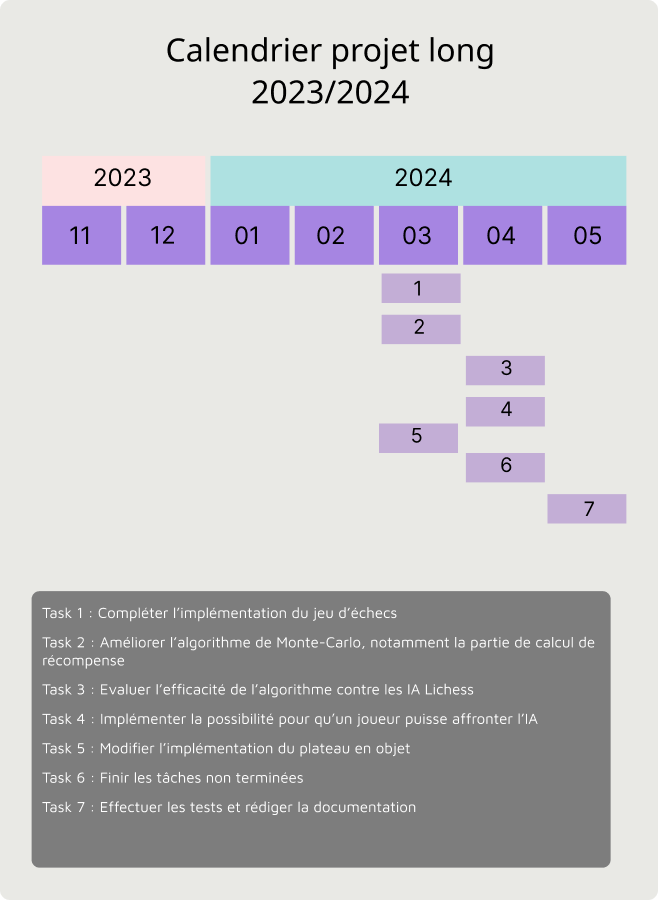
\includegraphics[width=0.8\linewidth]{Schedule.png}
  \caption{Figure d'organisation temporelle des tâches.}
  \label{fig:Schedule}
\end{figure}



\end{document}